% Prof. Dr. Ausberto S. Castro Vera
% UENF - CCT - LCMAT - Curso de Ciência da Computaçãoo
% Campos, RJ,  2023
% Disciplina: Paradigmas de Linguagens de Programação
% Aluno: Mariana Cossetti Dalfior

%%%*****************************************************************************************%%%
\chapter{Conceitos b\'{a}sicos da Linguagem Python}
%%%*****************************************************************************************%%%
Neste cap\'{\i}tulo ser\~{a}o apresentados os aspectos b\'{a}sicos da linguagem de programa\c{c}\~{a}o Python, incluindo atribui\c{c}\~{o}es, vari\'{a}veis, fun\c{c}\~{o}es, estruturas de controle, input/output e tipos de dados.

%%%=========================================================================================%%%
	\section{Vari\'{a}veis}
%%%=========================================================================================%%%
As vari\'{a}veis s\~{a}o elementos essenciais na programa\c{c}\~{a}o em Python, visto que s\~{a}o espa\c{c}os reservados na mem\'{o}ria que armazenam dados - desde n\'{u}mero e textos, at\'{e} objetos - que podem ser alterados durante a execu\c{c}\~{a}o de um programa. Em Python segundo \cite{Sousa2020} as vari\'{a}veis s\~{a}o tratadas como objetos, em que cada objeto receber\'{a} um determinado valor a ser armazenado ou um resultado obtido atrav\'{e}s de um comando. Para a cria\c{c}\~{a}o de uma vari\'{a}vel \'{e} necess\'{a}rio escolher um nome e atribuir a ela uma valor utilizando \textsl{'='}. Exemplos de vari\'{a}veis em Python: 
	
\begin{lstlisting}
>>> # variavel com str
>>> Nome = 'Mariana Cossetti Dalfior'

>>> # variavel com int
>>> Idade = 20

>>> # variavel com float
>>> Peso = 55
\end{lstlisting}

%%%.........................................................................................%%%
		\subsection{Regras de nomenclatura de uma vari\'{a}vel}
%%%.........................................................................................%%%
Existem algumas regras para nomear as vari\'{a}veis em Python. 

O que \'{e} permitido:
	\begin{itemize}
		\item Come\c{c}ar com uma letra ou com um sublinhado '\textsl{\_}'.
		\item O restante do nome pode receber letras, n\'{u}meros e sublinhados.
		\item Os nomes das vari\'{a}veis s\~{a}o sens\'{\i}veis a mai\'{u}sculas e min\'{u}sculas. Ent\~{a}o 'teste' e 'Teste' s\~{a}o nomes distintos de vari\'{a}veis.
	\end{itemize}
		
\begin{lstlisting}
>>> # Permitido
>>> nome
>>> Idade
>>> idade
>>> _bolo
>>> nota_1
\end{lstlisting}
		
		
O que n\~{a}o \'{e} permitidos:
	\begin{itemize}
		\item Come\c{c}ar com n\'{u}mero.
		\item Palavras-chave da linguagem utilizadas para fun\c{c}\~{o}es, como '\textsl{if}', '\textsl{else}', '\textsl{while}', '\textsl{for}', '\textsl{def}', '\textsl{class}' n\~{a}o podem ser empregues como nomes de vari\'{a}veis.
	\end{itemize}
		
\begin{lstlisting}
>>> # Nao permitido
>>> 1bolo
>>> 25_anos
>>> for
>>> %juros
\end{lstlisting}

%%%=========================================================================================%%%
	\section{Constantes}
%%%=========================================================================================%%%
Na linguagem de programa\c{c}\~{a}o Python n\~{a}o existe um tipo espec\'{\i}fico para as constantes como acontece em outras linguagens. Entretanto, de acordo com \cite{Sousa2020} \'{e} poss\'{\i}vel realizar a cria\c{c}\~{a}o de constantes atrav\'{e}s de uma conven\c{c}\~{a}o de nomenclatura, utilizando o nome da constante escrito em letras mai\'{u}sculas e no lugar dos espa\c{c}os utilizar o '\textsl{\_}'. Por\'{e}m, essa conven\c{c}\~{a}o n\~{a}o impossibilita que o valor da vari\'{a}vel seja modificado durante a execu\c{c}\~{a}o do programa, mas faz com que os programadores entendam e tratem essa vari\'{a}vel como constante. Exemplos de constantes em Python:

	
\begin{lstlisting}
>>> # Valor de Pi
>>> PI = 3.141592

>>> # Constante de Napier (base do logaritmo natural)
>>> NAPIER = 2.71828
\end{lstlisting}
	 
Ademais, existem m\'{o}dulos que possuem constantes j\'{a} pr\'{e}-definidas em Python, como o '\textsl{math}' que disp\~{o}em de \textsl{Pi} e a constante de \textsl{Euler}. Como acessar as constantes desse m\'{o}dulo são mostrados a seguir com o c\'{o}digo fonte \ref{fontecons} e o resultado \ref{resulcons} dos exemplos em Python:
	
\begin{lstlisting}
>>> # importando biblioteca
>>> import math
>>>
>>> # mostra pi
>>> print('O valor de Pi: {}' .format(math.pi))
O valor de Pi: 3.41592653589793
>>> 
>>> # mostra euler
>>> print('O valor de Euler: {}' .format(math.e))
O valor de Euler: 2.718281828459045
\end{lstlisting}

\begin{figure}[H]
\begin{center}
	\caption{C\'{o}digo fonte do exemplo de constantes} \label{fontecons}
	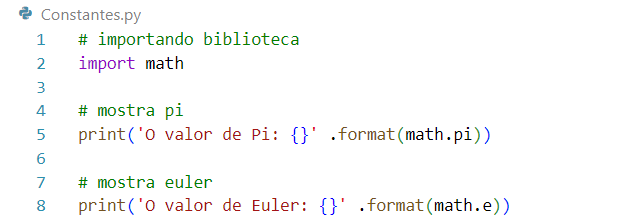
\includegraphics[width=12cm]{constantes} 
	\newline
	Fonte: Criado por Mariana Cossetti Dalfior
\end{center}
\end{figure}

\begin{figure}[H]
\begin{center}
	\caption{Resultado do c\'{o}digo fonte do exemplo de constantes} \label{resulcons}
	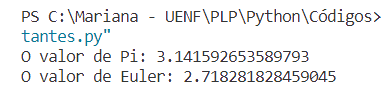
\includegraphics[width=9cm]{resulconstantes} 
	\newline
	Fonte: Criado por Mariana Cossetti Dalfior
\end{center}
\end{figure}

%%%=========================================================================================%%%
	\section{Entrada e Sa\'{\i}da de Dados}
%%%=========================================================================================%%%
Segundo \cite{Yoon2022} a entrada e sa\'{\i}da de dados em Python \'{e} realizada atrav\'{e}s da utiliza\c{c}\~{a}o de uma biblioteca padr\~{a}o.

%%%.........................................................................................%%%
\subsection{Input}
%%%.........................................................................................%%%

A entrada de dados \'{e} feita por meio da fun\c{c}\~{a}o \textsl{'input()'}, permitindo que seja inserido valores ou informa\c{c}\~{o}es - sejam elas strings, n\'{u}meros e  booleanos - pelos usu\'{a}rios enquanto o programa \'{e} executado. Essa fun\c{c}\~{a}o solicita que o usu\'{a}rio digite uma informa\c{c}\~{a}o - a execu\c{c}\~{a}o do programa fica pausada at\'{e} que essa informa\c{c}\~{a}o seja retornada - e ent\~{a}o a armazena em uma vari\'{a}vel. Por\'{e}m todos os dados que s\~{a}o inseridos usando essa fun\c{c}\~{a}o s\~{a}o tratados como strings, ent\~{a}o para transform\'{a}-los em outro tipo ser\'{a} necess\'{a}rio a utiliza\c{c}\~{a}o do \textsl{'int()'} ou \textsl{'float()'}. A seguir \'{e} poss\'{\i}vel observar o c\'{o}digo fonte \ref{fonteinput} e o resultado \ref{resulinput} dos exemplos em Python:

\begin{lstlisting}
>>> # entrada em formato de str
>>> aluno = input('Nome: ')
>>>
>>> # entrada em formato de int
>>> matricula = int(input('Numero de matricula: '))
>>>
>>> # entrada em formato de float
>>> nota = float(input('Nota da prova: '))
>>>
\end{lstlisting}

\begin{figure}[H]
	\begin{center}
		\caption{C\'{o}digo fonte do exemplo de input} \label{fonteinput}
		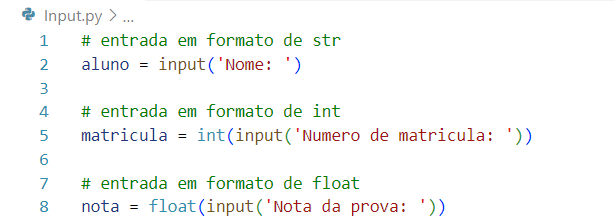
\includegraphics[width=12cm]{input} 
		\newline
		Fonte: Criado por Mariana Cossetti Dalfior
	\end{center}
\end{figure}

\begin{figure}[H]
	\begin{center}
		\caption{Resultado do c\'{o}digo fonte do exemplo de input} \label{resulinput}
		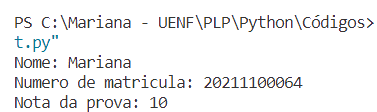
\includegraphics[width=9cm]{resulinput} 
		\newline
		Fonte: Criado por Mariana Cossetti Dalfior
	\end{center}
\end{figure}

%%%.........................................................................................%%%
\subsection{Output}
%%%.........................................................................................%%%

A sa\'{\i}da de dados em Python \'{e} comumente executada pela fun\c{c}\~{a}o \textsl{'print()'}, possuindo como encargo exibir na tela as informa\c{c}\~{a}o geradas pelo programa para o usu\'{a}rio - seja ela uma mensagem, valores e informa\c{c}\~{o}es. EA seguir \'{e} poss\'{\i}vel observar o c\'{o}digo fonte \ref{fontoutput} e o resultado \ref{resuloutput} dos exemplos de sa\'{\i}da de dados em Python:

\begin{lstlisting}
>>> # saida de uma frase
>>> print('Um prato de trigo para tres tigres tristes.')
Um prato de trigo para tres tigres tristes.

>>> # saida do valor de uma variavel
>>> aluno = "Mariana"
>>> matricula = 20211100064
>>> print('{} tem a matricula {}' .format(aluno, matricula))
Mariana tem a matricula 2021110064
\end{lstlisting}

\begin{figure}[H]
	\begin{center}
		\caption{C\'{o}digo fonte do exemplo de output} \label{fonteoutput}
		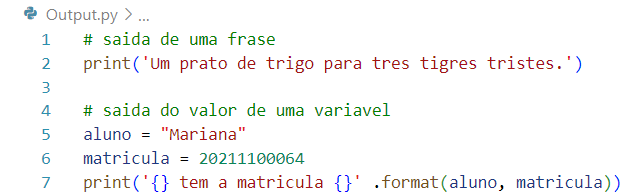
\includegraphics[width=12cm]{output} 
		\newline
		Fonte: Criado por Mariana Cossetti Dalfior
	\end{center}
\end{figure}

\begin{figure}[H]
	\begin{center}
		\caption{Resultado do c\'{o}digo fonte do exemplo de output} \label{resuloutput}
		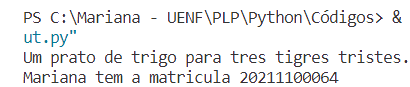
\includegraphics[width=9cm]{resuloutput} 
		\newline
		Fonte: Criado por Mariana Cossetti Dalfior
	\end{center}
\end{figure}
	
No \'{u}ltimo exemplo foi utilizado o \textsl{'format()'}, utilizado para substituir os espa\c{c}os que foram reservados para as vari\'{a}veis fornecidas como argumento.


%%%=========================================================================================%%%
    \section{Tipos de Dados B\'{a}sicos}
%%%=========================================================================================%%%

Os tipos de dados b\'{a}sicos s\~{a}o utilizados para realizar as opera\c{c}\~{o}es b\'{a}sicas de acordo com \cite{Miller2019}. Esses podem ser divididos n\~{a}o seguintes tipos de dados:

%%%.........................................................................................%%%
            \subsection{String} \label{subsec:str}
%%%.........................................................................................%%%
As strings em Python s\~{a}o uma parte fundamental da linguagem, pois representam uma sequ\^{e}ncia de caracteres - podem ser letras, s\'{\i}mbolos, letras e espa\c{c}os em branco. Elas s\~{a}o criadas utilizando aspas simples e duplas. A seguir \'{e} poss\'{\i}vel observar o c\'{o}digo fonte \ref{fontestring} e o resultado \ref{resulstring} dos exemplos de strings em Python:

\begin{lstlisting}
>>> # Usando aspas simples
>>> exemStr = 'Vasco da Gama'
>>> print (exemStr)  
Vasco da Gama

>>> # Usando aspas duplas
>>> exemStr2 = "Vasco da Gama o maior do Rio!"
>>> print (exemStr2)
Vasco da Gama o maior do Rio!
\end{lstlisting}

\begin{figure}[H]
	\begin{center}
		\caption{C\'{o}digo fonte do exemplo de strings} \label{fontestring}
		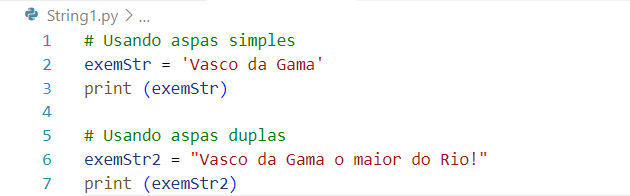
\includegraphics[width=12cm]{string1} 
		\newline
		Fonte: Criado por Mariana Cossetti Dalfior
	\end{center}
\end{figure}

\begin{figure}[H]
	\begin{center}
		\caption{Resultado do c\'{o}digo fonte do exemplo de strings} \label{resulstring}
		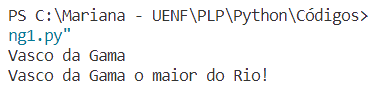
\includegraphics[width=9cm]{resulstring1} 
		\newline
		Fonte: Criado por Mariana Cossetti Dalfior
	\end{center}
\end{figure}

Em Python as strings suportam diversos m\'{e}todos embutidos - que servem para a formata\c{c}\~{a}o e manipula\c{c}\~{a}o das mesmas - como \textsl{'.upper()'} e \textsl{'.lower()'}. A seguir \'{e} poss\'{\i}vel observar o c\'{o}digo fonte \ref{fontestrings2} e o resultado \ref{resulstrings2} dos exemplos de aplica\c{c}\~{a}o desses m\'{e}todos:

\begin{lstlisting}
>>> # Usando o .upper()
>>> exemStr = 'Gabriel Pec'
>>> print(exemStr.upper())
GABRIEL PEC

>>> # Usando o .lower()
>>> exemStr2 = 'Leo Pele'
>>> print(exemStr2.lower())
leo pele
\end{lstlisting}

\begin{figure}[H]
	\begin{center}
		\caption{C\'{o}digo fonte do exemplo de \textsl{.upper} e \textsl{.lower}} \label{fontestrings2}
		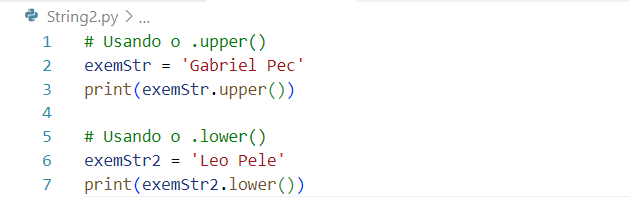
\includegraphics[width=12cm]{string2} 
		\newline
		Fonte: Criado por Mariana Cossetti Dalfior
	\end{center}
\end{figure}

\begin{figure}[H]
	\begin{center}
		\caption{Resultado do c\'{o}digo fonte do exemplo de \textsl{.upper} e \textsl{.lower}} \label{resulstrings2}
		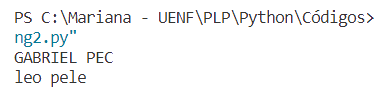
\includegraphics[width=9cm]{resulstring2} 
		\newline
		Fonte: Criado por Mariana Cossetti Dalfior
	\end{center}
\end{figure}

A seguir \'{e} poss\'{\i}vel observar o c\'{o}digo fonte \ref{fonteconcatenacao1}, \ref{fonteconcatenacao2} e o resultado \ref{resulconcatenacao1}, \ref{resulconcatenacao2} dos exemplos de manipula\c{c}\~{a}o de Strings utilizadas em Python:

\begin{itemize}
  \item \textit{Concatena\c{c}\~{a}o de strings}\newline
        Duas ou mais strings podem ser concatenadas utilizando o operador \textsl{'+'}.
        
\begin{lstlisting}
>>> # Concatenando 2 strings
>>> print ("Cruz" + " de Malta")
Cruz de Malta
\end{lstlisting}

\begin{figure}[H]
	\begin{center}
		\caption{C\'{o}digo fonte do exemplo de concatena\c{c}\~{a}o de strings} \label{fonteconcatenacao1}
		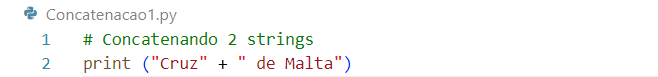
\includegraphics[width=12cm]{concatenacao1} 
		\newline
		Fonte: Criado por Mariana Cossetti Dalfior
	\end{center}
\end{figure}

\begin{figure}[H]
	\begin{center}
		\caption{C\'{o}digo fonte do exemplo de concatena\c{c}\~{a}o de strings} \label{resulconcatenacao1}
		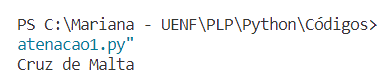
\includegraphics[width=9cm]{resulconcatenacao1} 
		\newline
		Fonte: Criado por Mariana Cossetti Dalfior
	\end{center}
\end{figure}
    
Outra forma de juntar strings e de forma mais eficiente \'{e} atrav\'{e}s do uso do m\'{e}todo \textsl{'.join()'}, capaz de concatenar um lista de strings em apenas uma string.

\begin{lstlisting}
>>> # Concatenando 2 nomes
>>> jogadores = ["Jair", "Andrey"]
>>> print( ", ".join(jogadores))
Jair, Andrey
\end{lstlisting} 

\begin{figure}[H]
	\begin{center}
		\caption{C\'{o}digo fonte do exemplo de concatena\c{c}\~{a}o de lista de strings} \label{fonteconcatenacao2}
		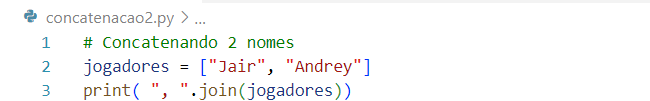
\includegraphics[width=12cm]{concatenacao2} 
		\newline
		Fonte: Criado por Mariana Cossetti Dalfior
	\end{center}
\end{figure}

\begin{figure}[H]
	\begin{center}
		\caption{Resultado do c\'{o}digo fonte do exemplo de concatena\c{c}\~{a}o de lista de strings} \label{resulconcatenacao2}
		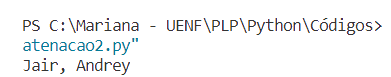
\includegraphics[width=9cm]{resulconcatenacao2} 
		\newline
		Fonte: Criado por Mariana Cossetti Dalfior
	\end{center}
\end{figure}

\item \textit{Operador de indexa\c{c}\~{a}o}\newline
Qualquer elemento individual de uma lista, string ou tupla pode ser acessado com o operador de indexa\c{c}\~{a}o \textsl{'[]'}, usando apenas o \'{\i}ndice entre os colchetes depois da vari\'{a}vel que armazena essa sequ\^{e}ncia. Existem duas formas de indexar os caracteres de um string em Python: \newline
\begin{description}
	  \item[Index com inteiros positivos] come\c{c}ando da esquerda para direita utilizando o 0 como index do primeiro caractere da sequ\^{e}ncia.
	  \item[Index com inteiros negativos] come\c{c}ando da direita para a esquerda utilizando o -1 para iniciar o index sendo ele o \'{u}ltimo elemento da sequ\^{e}ncia, -2 o pen\'{u}ltimo elemento, e assim consecutivamente.
\end{description}

A seguir \'{e} poss\'{\i}vel observar o c\'{o}digo fonte \ref{fontefrase} e o resultado \ref{resulfrase} do exemplo de indexa\c{c}\~{a}o em Python:

\begin{lstlisting}
>>> # indexando com inteiros positivos
>>> frase = "Vasco da Gama"
>>> print(frase[0:5])
Vasco
\end{lstlisting}

\begin{figure}[H]
	\begin{center}
		\caption{C\'{o}digo fonte do exemplo de indexa\c{c}\~{a}o} \label{fontefrase}
		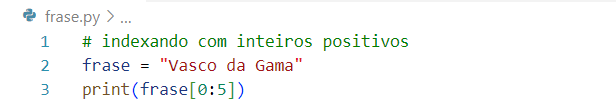
\includegraphics[width=12cm]{frase} 
		\newline
		Fonte: Criado por Mariana Cossetti Dalfior
	\end{center}
\end{figure}

\begin{figure}[H]
	\begin{center}
		\caption{Resultado do c\'{o}digo fonte do exemplo de indexa\c{c}\~{a}o} \label{resulfrase}
		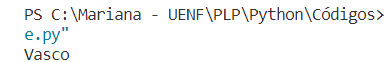
\includegraphics[width=9cm]{resulfrase} 
		\newline
		Fonte: Criado por Mariana Cossetti Dalfior
	\end{center}
\end{figure}

\item \textit{Formata\c{c}\~{a}o de strings}\newline
Strings podem ser formatadas de forma din\^{a}mica com base em valores vari\'{a}veis atrav\'{e}s do m\'{e}todo \textsl{'.format()'}.Esse m\'{e}todo permite a cria\c{c}\~{a}o de strings com espa\c{c}o reservado para serem preenchidos com valores vari\'{a}veis. A seguir \'{e} poss\'{\i}vel observar o c\'{o}digo fonte \ref{fonteformat}, \ref{fonteformat2} e o resultado \ref{resulformat}, \ref{resulformat2} do exemplo da formata\c{c}\~{a}o em Python:
		
\begin{lstlisting}
>>> nome = "Pedro Raul"
>>> idade = 26
>>> print("O jogador {} possui {} anos." .format(nome, idade))
O jogador Pedro Raul possui 26 anos.
\end{lstlisting}
	
\begin{figure}[H]
	\begin{center}
		\caption{C\'{o}digo fonte do exemplo de formata\c{c}\~{a}o de strings} \label{fonteformat}
		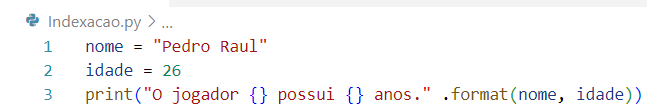
\includegraphics[width=12cm]{format} 
		\newline
		Fonte: Criado por Mariana Cossetti Dalfior
	\end{center}
\end{figure}

\begin{figure}[H]
	\begin{center}
		\caption{Resultado do c\'{o}digo fonte do exemplo de formata\c{c}\~{a}o de strings} \label{resulformat}
		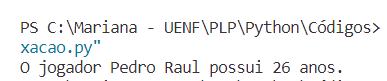
\includegraphics[width=9cm]{resulformat} 
		\newline
		Fonte: Criado por Mariana Cossetti Dalfior
	\end{center}
\end{figure}
	
Em vers\~{o}es mais atuais do Python existe outra tipo de formata\c{c}\~{a}o, utilizando uma forma mais intuitiva e simples. 
		
\begin{lstlisting}
>>> nome = "Pedro Raul"
>>> idade = 26
>>> print("O jogador", nome, "possui", idade, "anos.")
O jogador Pedro Raul possui 26 anos.
\end{lstlisting}

\begin{figure}[H]
	\begin{center}
		\caption{C\'{o}digo fonte do outro exemplo de formata\c{c}\~{a}o de strings} \label{fonteformat2}
		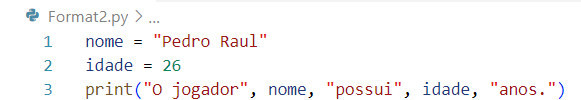
\includegraphics[width=12cm]{format2} 
		\newline
		Fonte: Criado por Mariana Cossetti Dalfior
	\end{center}
\end{figure}

\begin{figure}[H]
	\begin{center}
		\caption{Resultado do c\'{o}digo fonte do outro exemplo de formata\c{c}\~{a}o de strings} \label{resulformat2}
		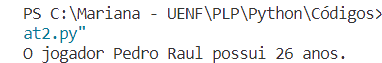
\includegraphics[width=9cm]{resulformat2} 
		\newline
		Fonte: Criado por Mariana Cossetti Dalfior
	\end{center}
\end{figure}
		
    \end{itemize}

%%%.........................................................................................%%%
\subsection{Opera\c{c}\~{o}es l\'{o}gicas}
%%%.........................................................................................%%%
Os operadores l\'{o}gicos s\~{a}o utilizados para realizar opera\c{c}\~{o}es sobre dados booleanos(l\'{o}gicos). Os resultados dessas opera\c{c}\~{o}es podem retornar \textsl{true}(verdadeiro) ou  \textsl{false}(falso). A seguir ser\~{a}o mostrados quais s\~{a}o esses operadores e o que eles significam. \newline

\begin{table}[H]
	\centering
	{\renewcommand\arraystretch{1.25}
		\begin{tabular}{ l l }
			\multicolumn{1}{p{3cm}|} {\centering\textbf{Opera\c{c}\~{o}es}} &
			\multicolumn{1}{p{3cm}}{\centering\textbf{Operador}}
			\\    
			\cline{1-1}\cline{2-2}
			\multicolumn{1}{p{3cm}|}{Menor que} &
			\multicolumn{1}{p{3cm}}{\centering < }
			\\  
			\multicolumn{1}{p{3cm}|}{Maior que} &
			\multicolumn{1}{p{3cm}}{\centering >}
			\\   
			\multicolumn{1}{p{3cm}|}{Menor ou igual} &
			\multicolumn{1}{p{3cm}}{\centering <= }
			\\   
			\multicolumn{1}{p{3cm}|}{Maior ou igual} &
			\multicolumn{1}{p{3cm}}{\centering >=}
			\\   
			\multicolumn{1}{p{3cm}|}{Igual} &
			\multicolumn{1}{p{3cm}}{\centering ==}
			\\   
			\multicolumn{1}{p{3cm}|}{Diferente de} &
			\multicolumn{1}{p{3cm}}{\centering !=}
			\\  
	\end{tabular} }		
	\caption{Opera\c{c}\~{o}es l\'{o}gicas em Python}
\end{table}

A seguir \'{e} poss\'{\i}vel observar o c\'{o}digo fonte \ref{fontelogicas} e o resultado \ref{resullogicas} do exemplo da utiliza\c{c}\~{a}o de opera\c{c}\~{o}es l\'{o}gicas: 
\begin{lstlisting}
	>>> # Menor que
	>>> print(35 < 12)
	False
	>>> # Maior que
	>>> print(64 > 40)
	True
	>>> # Menor ou igual
	>>> print(120 <= 120)
	True
	>>> # Maior ou igual que
	>>> print(32 >= 165)
	False
	>>> # Igual
	>>> print(15 == 80)
	False
	>>> # Diferente de
	>>> print(30 != 15)
	True
\end{lstlisting}

\begin{figure}[H]
	\begin{center}
		\caption{C\'{o}digo fonte do exemplo de opera\c{c}\~{o}es l\'{o}gicas} \label{fontelogicas}
		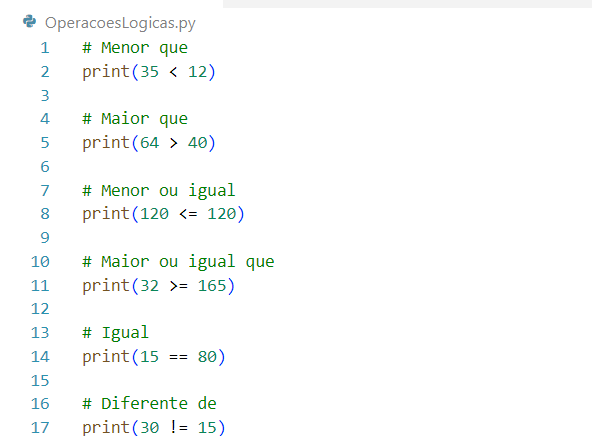
\includegraphics[width=12cm]{logicas} 
		\newline
		Fonte: Criado por Mariana Cossetti Dalfior
	\end{center}
\end{figure}

\begin{figure}[H]
	\begin{center}
		\caption{Resultado do c\'{o}digo fonte do exemplo de opera\c{c}\~{o}es l\'{o}gicas} \label{resullogicas}
		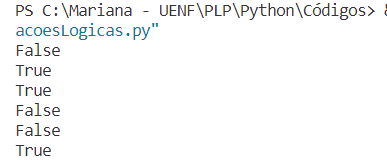
\includegraphics[width=9cm]{resullogicas} 
		\newline
		Fonte: Criado por Mariana Cossetti Dalfior
	\end{center}
\end{figure}

%%%.........................................................................................%%%
		\subsection{N\'{u}meros Inteiros}
%%%.........................................................................................%%%
Os n\'{u}meros inteiros em Python representam todos os n\'{u}meros inteiros positivos, negativos e o zero. Eles s\~{a}o armazenados como objetos inteiros e n\~{a}o possuem limite para o tamanho dos n\'{u}meros que podem ser armazenados em uma vari\'{a}vel inteira. 
Exemplo de n\'{u}mero inteiro em Python:

\begin{lstlisting}
>>> # inteiro positivo
>>> c = 10

>>> # inteiro negativo
>>> r = -200

>>> # zero
>>> v = 0
\end{lstlisting}

Em geral, uma express\~{a}o Python \'{e} uma combina\c{c}\~{a}o de operadores e operandos. Quando avaliamos uma express\~{a}o, obtemos um resultado. Nos pr\'{o}ximos exemplos s\~{a}o realizadas opera\c{c}\~{o}es aritm\'{e}ticas com n\'{u}meros inteiros, como adi\c{c}\~{a}o \textsl{'+'}, subtra\c{c}\~{a}o \textsl{'-'}, multiplica\c{c}\~{a}o \textsl{'*'}, divis\~{a}o \textsl{'/'}, resto da divis\~{a}o \textsl{'\%'} e divis\~{a}o inteira \textsl{'//'} . Ademais, talvez voc\^{e} esteja mais acostumado com \textsl{'x'} e \textsl{'÷'} para multiplica\c{c}\~{a}o e divis\~{a}o, mas em Python e quase todas as outras linguagens de programa\c{c}\~{a}o usam \textsl{'*'} e \textsl{'/'}.  A seguir \'{e} poss\'{\i}vel observar o c\'{o}digo fonte \ref{fonteinteiros} e o resultado \ref{resulinteiros} dos exemplos de n\'{u}mero inteiro em Python:

\begin{lstlisting}
>>> # variaveis 
>>> v = 14
>>> g = 3
>>> 
>>> # soma de inteiros
>>> print(v + g)
17
>>> # subtracao de inteiros
>>> print(v - g) 
11
>>> # multiplicacao de inteiros
>>> print(v * g)
42
>>> # divisao de inteiros
>>> print(v / g)
4.666666666666
>>> # resto da divisao de inteiros
>>> print(v % g)
2
>>> #divisao inteira de inteiros
>>> print(v // g) 
4
\end{lstlisting}

\begin{figure}[H]
	\begin{center}
		\caption{C\'{o}digo fonte do exemplo de opera\c{c}\~{o}es com n\'{u}meros inteiros} \label{fonteinteiros}
		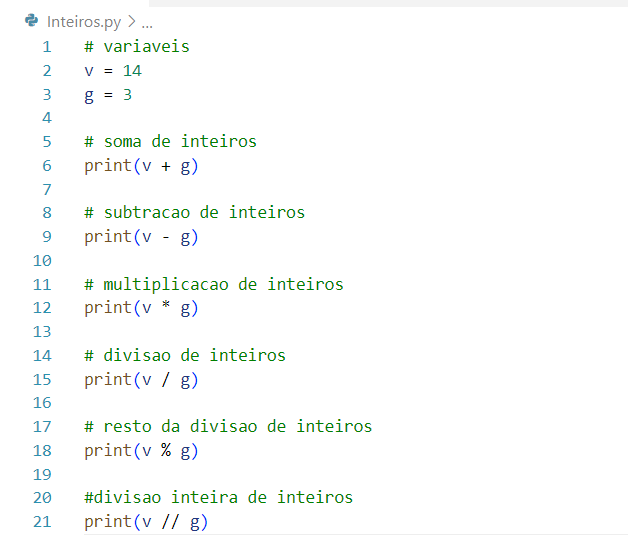
\includegraphics[width=12cm]{inteiros} 
		\newline
		Fonte: Criado por Mariana Cossetti Dalfior
	\end{center}
\end{figure}

\begin{figure}[H]
	\begin{center}
		\caption{Resultado do c\'{o}digo fonte do exemplo de opera\c{c}\~{o}es com n\'{u}meros inteiros} \label{resulinteiros}
		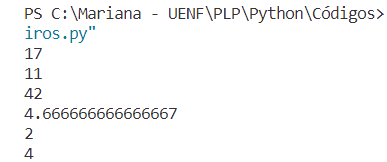
\includegraphics[width=9cm]{resulinteiros} 
		\newline
		Fonte: Criado por Mariana Cossetti Dalfior
	\end{center}
\end{figure}


%%%.........................................................................................%%%
		\subsection{N\'{u}meros de Ponto Flutuante}
%%%.........................................................................................%%%

Os n\'{u}meros de ponto flutuante s\~{a}o a aproxima\c{c}\~{a}o do Python do que voc\^{e} chamou de n\'{u}meros reais nas aula de matem\'{a}tica. Os n\'{u}meros de ponto flutuante s\~{a}o uma aproxima\c{c}\~{a}o porque, diferentemente dos n\'{u}meros reais, os n\'{u}meros de ponto flutuante n\~{a}o podem ter um n\'{u}mero infinito de d\'{\i}gitos ap\'{o}s o ponto decimal. No Python, os n\'{u}meros de ponto flutuante s\~{a}o armazenados como objetos float e s\~{a}o aproximados de forma bin\'{a}ria, podendo apresentar algumas imprecis\~{o}es com valores decimais exatos. A seguir \'{e} poss\'{\i}vel observar o c\'{o}digo fonte \ref{fontefloat1} e o resultado \ref{resulfloat1} do exemplo de n\'{u}meros de ponto flutuante em Python:

\begin{lstlisting}
>>> # variaveis
>>> v = 0.5
>>> g = 0.2
>>> # soma de floats
>>> f = v + g
>>> print(f)
0.7
\end{lstlisting}

\begin{figure}[H]
	\begin{center}
		\caption{C\'{o}digo fonte do exemplo com n\'{u}meros de ponto flutuante} \label{fontefloat1}
		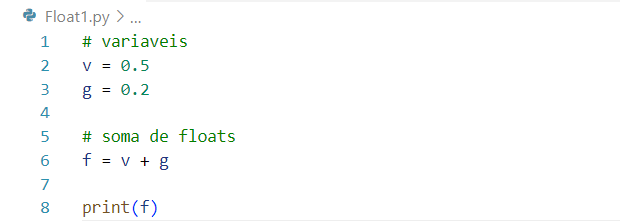
\includegraphics[width=12cm]{float1} 
		\newline
		Fonte: Criado por Mariana Cossetti Dalfior
	\end{center}
\end{figure}

\begin{figure}[H]
	\begin{center}
		\caption{Resultado do c\'{o}digo fonte do exemplo com n\'{u}meros de ponto flutuante} \label{resulfloat1}
		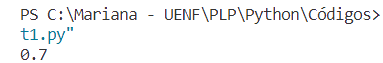
\includegraphics[width=9cm]{resulfloat1} 
		\newline
		Fonte: Criado por Mariana Cossetti Dalfior
	\end{center}
\end{figure}

Do mesmo modo que os n\'{u}meros inteiros, \'{e} poss\'{\i}vel realizar opera\c{c}\~{o}es aritm\'{e}ticas com n\'{u}meros de ponto flutuante, como adi\c{c}\~{a}o \textsl{'+'}, subtra\c{c}\~{a}o \textsl{'-'}, multiplica\c{c}\~{a}o \textsl{'*'}, divis\~{a}o \textsl{'/'}, resto da divis\~{a}o \textsl{'\%'} e divis\~{a}o inteira \textsl{'//'}. A seguir \'{e} poss\'{\i}vel observar o c\'{o}digo fonte \ref{fontefloat2} e o resultado \ref{resulfloat2} do exemplo de opera\c{c}\~{o}es aritm\'{e}ticas com n\'{u}meros de ponto flutuante em Python:

\begin{lstlisting}
>>> # variaveis 
>>> v = 10.33
>>> g = 5
>>>
>>> # soma de floats
>>> print(v + g)
15.33
>>> # subtracao de floats
>>> print(v - g) 
5.33
>>> # multiplicacao de floats
>>> print(v * g)
51.65
>>> # divisao de floats
>>> print(v / g)
2.066
>>> # resto da divisao de floats
>>> print(v % g)
0.3300000000007
>>> #divisao inteira de floats
>>> print(v // g) 
2.0
\end{lstlisting}

\begin{figure}[H]
	\begin{center}
		\caption{C\'{o}digo fonte do exemplo de opera\c{c}\~{o}es com n\'{u}meros de ponto flutuante} \label{fontefloat2}
		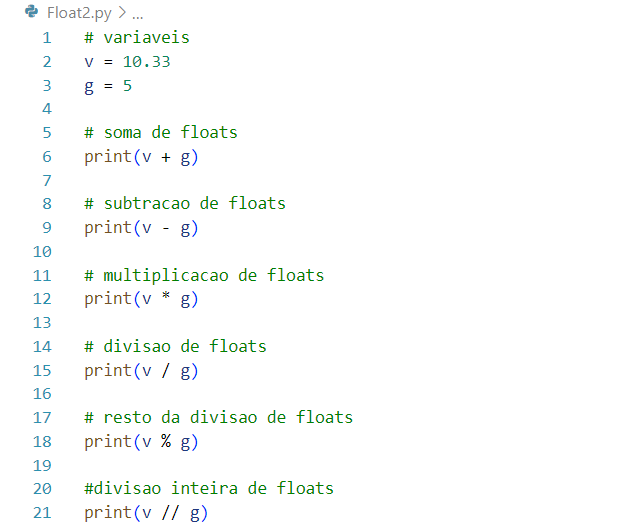
\includegraphics[width=12cm]{float2} 
		\newline
		Fonte: Criado por Mariana Cossetti Dalfior
	\end{center}
\end{figure}

\begin{figure}[H]
	\begin{center}
		\caption{Resultado do c\'{o}digo fonte do exemplo de opera\c{c}\~{o}es com n\'{u}meros de ponto flutuante} \label{resulfloat2}
		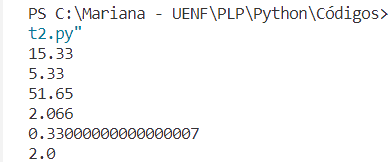
\includegraphics[width=9cm]{resulfloat2} 
		\newline
		Fonte: Criado por Mariana Cossetti Dalfior
	\end{center}
\end{figure}

%%%.........................................................................................%%%
\subsection{N\'{u}meros complexos}
%%%.........................................................................................%%%

O \'{u}ltimo tipo num\'{e}rico primitivo em Python \'{e} o n\'{u}mero complexo. Como voc\^{e} pode se recordar, os n\'{u}meros complexos t\^{e}m duas partes: uma parte real e uma parte imagin\'{a}ria. No Python, um n\'{u}mero complexo \'{e} exibido como \textsl{real} + \textsl{imagin\'{a}rio}j. A seguir \'{e} poss\'{\i}vel observar o c\'{o}digo fonte \ref{fontecomplexos} e o resultado \ref{resulcomplexos} do exemplo de n\'{u}meros complexos em Python:

\begin{lstlisting}
>>> # Numeros complexos
>>> print(100000000000000000000000000 * 3.4)
3.40000000000000003e+26 
>>> print(5 + 4+3j)
(9 + 3j)
>>>
\end{lstlisting}

\begin{figure}[H]
	\begin{center}
		\caption{C\'{o}digo fonte do exemplo com n\'{u}meros complexos} \label{fontecomplexos}
		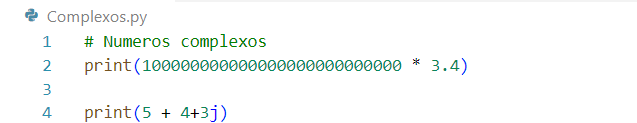
\includegraphics[width=12cm]{complexos} 
		\newline
		Fonte: Criado por Mariana Cossetti Dalfior
	\end{center}
\end{figure}

\begin{figure}[H]
	\begin{center}
		\caption{Resultado do c\'{o}digo fonte do exemplo com n\'{u}meros complexos} \label{resulcomplexos}
		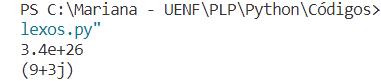
\includegraphics[width=9cm]{resulcomplexos} 
		\newline
		Fonte: Criado por Mariana Cossetti Dalfior
	\end{center}
\end{figure}


%%%.........................................................................................%%%
		\subsection{Booleanos}
%%%.........................................................................................%%%
 Os booleanos s\~{a}o escritos como palavras-chave '\textsl{True}' e '\textsl{False}', sem aspas e com a primeira letra em mai\'{u}scula. S\~{a}o utilizados em express\~{o}es l\'{o}gicas e em estruturas de controle de fluxo, como o \textsl{if} e o \textsl{while}, podendo ser combinados com o \textsl{and}, \textsl{or} e \textsl{not}. A seguir \'{e} poss\'{\i}vel observar o c\'{o}digo fonte \ref{fontebool} e o resultado \ref{resulbool} do exemplo de booleano usado em um \textsl{if} com \textsl{and} :

\begin{lstlisting}
>>> # variaveis
>>> v = 6
>>> g = 12
>>> 
>>> if v > 5 and g > 3:
>>> 	print("{} maior que 5 e {} e maior que 3" .format(v, g))
6 e maior que 5 e 12 maior que 3
\end{lstlisting}

\begin{figure}[H]
	\begin{center}
		\caption{C\'{o}digo fonte do exemplo com n\'{u}meros booleanos em um \textsl{if}} \label{fontebool}
		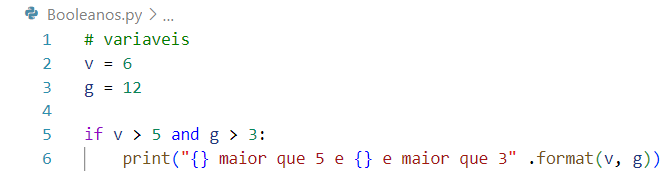
\includegraphics[width=12cm]{bool} 
		\newline
		Fonte: Criado por Mariana Cossetti Dalfior
	\end{center}
\end{figure}

\begin{figure}[H]
	\begin{center}
		\caption{Resultado do c\'{o}digo fonte do exemplo com n\'{u}meros booleanos em um \textsl{if}} \label{resulbool}
		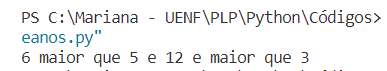
\includegraphics[width=9cm]{resulbool} 
		\newline
		Fonte: Criado por Mariana Cossetti Dalfior
	\end{center}
\end{figure}

Ademais,  \'{e} poss\'{\i}vel converter qualquer valor ou express\~{a}o em um booleano utilizando uma fun\c{c}\~{a}o chamada \textsl{'bool()'}.Essa fun\c{c}\~{a}o retorna '\textsl{False}' caso o valor for considerado "vazio", e '\textsl{True}' caso contr\'{a}rio. A seguir \'{e} poss\'{\i}vel observar o c\'{o}digo fonte \ref{fontebool2} e o resultado \ref{resulbool2} do exemplo: 

\begin{lstlisting}
>>> print(bool(0))       
False
>>> print(bool(1898))       
True
>>> print(bool(""))      
False
>>> print(bool("Vasco")) 
True
\end{lstlisting}

\begin{figure}[H]
	\begin{center}
		\caption{C\'{o}digo fonte do exemplo com n\'{u}meros booleanos} \label{fontebool2}
		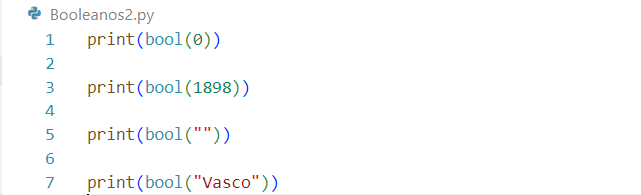
\includegraphics[width=12cm]{bool2} 
		\newline
		Fonte: Criado por Mariana Cossetti Dalfior
	\end{center}
\end{figure}

\begin{figure}[H]
	\begin{center}
		\caption{Resultado do c\'{o}digo fonte do exemplo com n\'{u}meros booleanos} \label{resulbool2}
		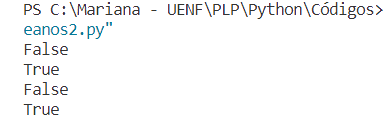
\includegraphics[width=9cm]{resulbool2} 
		\newline
		Fonte: Criado por Mariana Cossetti Dalfior
	\end{center}
\end{figure}

Em resumo, foi evidenciado que o Python oferece suporte a v\'{a}rios tipos diferentes de objetos primitivos: n\'{u}meros inteiros, n\'{u}meros de ponto flutuante, n\'{u}meros complexos, n\'{u}meros booleanos, Strings e as opera\c{c}\~{o}es l\'{o}gicas.

%%%=========================================================================================%%%
    \section{Estrutura de Controle e Fun\c{c}\~{o}es}
%%%=========================================================================================%%%
As estruturas de controle e fun\c{c}\~{o}es s\~{a}o elementos fundamentais da programa\c{c}\~{a}o em Python. A seguir ser\~{a}o mostradas algumas dessas estruturas segundo \cite{Guttag2021}: 
%%%.........................................................................................%%%
            \subsection{O comando \textsl{If}}
%%%.........................................................................................%%%
O comando "\textsl{if}" em Python \'{e} uma estrutura de controle que permite executar determinado bloco de c\'{o}digo se uma determinada condi\c{c}\~{a}o for verdadeira. A sintaxe b\'{a}sica em Python \'{e} a seguinte:
\begin{lstlisting}
>>> if condicao:
>>> 	# bloco de codigo
\end{lstlisting}	

A seguir \'{e} poss\'{\i}vel observar o c\'{o}digo fonte \ref{fonteif} e o resultado \ref{resulif} do exemplo com aplica\c{c}\~{a}o em Python:

\begin{lstlisting}
>>> # variavel
>>> v = 10
>>> 
>>> if v > 5:
>>> 	print("Gigante da Colina")
Gigante da Colina
\end{lstlisting}	

\begin{figure}[H]
	\begin{center}
		\caption{C\'{o}digo fonte do exemplo do uso do \textsl{if}} \label{fonteif}
		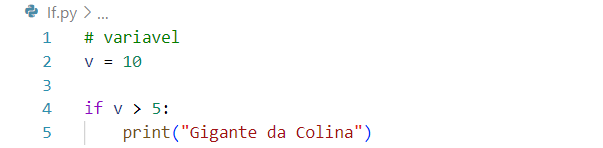
\includegraphics[width=12cm]{if} 
		\newline
		Fonte: Criado por Mariana Cossetti Dalfior
	\end{center}
\end{figure}

\begin{figure}[H]
	\begin{center}
		\caption{Resultado do c\'{o}digo fonte do exemplo do uso do \textsl{if}} \label{resulif}
		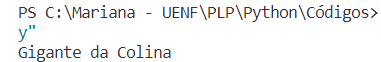
\includegraphics[width=9cm]{resulif} 
		\newline
		Fonte: Criado por Mariana Cossetti Dalfior
	\end{center}
\end{figure}
%%%.........................................................................................%%%
			\subsection{O comando \textsl{Else}}
%%%.........................................................................................%%%
O comando '\textsl{else}' \'{e} sempre utilizado em conjunto com o '\textsl{if}' para fornecer uma alternativa caso a condi\c{c}\~{a}o do \textsl{if} n\~{a}o seja verdadeira. Dessa forma, o bloco de c\'{o}digo dentro do \textsl{else} s\'{o} ser\'{a} executado se a condi\c{c}\~{a}o do \textsl{if} for falsa. A sintaxe b\'{a}sica em Python \'{e} a seguinte:
\begin{lstlisting}
>>> if condicao:
>>> 	# bloco de codigo a ser executado se a condicao for 
>>> 	# verdadeira
>>> else:
>>> 	# bloco de codigo a ser executado se a condicao for 
>>> 	# falsa
\end{lstlisting}	

A seguir \'{e} poss\'{\i}vel observar o c\'{o}digo fonte \ref{fonteelse} e o resultado \ref{resulelse} do exemplo com aplica\c{c}\~{a}o em Python:

\begin{lstlisting}
>>> # variavel
>>> v = 12
>>>
>>> if v % 2 == 0:
>>> 	print("O numero e par")
>>> else:
>>> 	print("O numero e impar")
O numero e par
\end{lstlisting}	

\begin{figure}[H]
\begin{center}
	\caption{C\'{o}digo fonte do exemplo do uso do \textsl{else}} \label{fonteelse}
	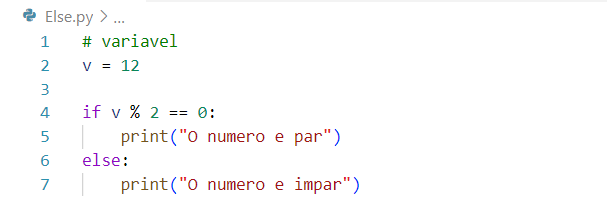
\includegraphics[width=12cm]{else} 
	\newline
	Fonte: Criado por Mariana Cossetti Dalfior
\end{center}
\end{figure}

\begin{figure}[H]
\begin{center}
	\caption{Resultado do c\'{o}digo fonte do exemplo do uso do \textsl{else}} \label{resulelse}
	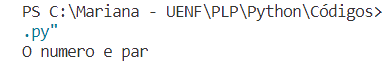
\includegraphics[width=9cm]{resulelse} 
	\newline
	Fonte: Criado por Mariana Cossetti Dalfior
\end{center}
\end{figure}

%%%.........................................................................................%%%
			\subsection{O comando \textsl{Elif}}
%%%.........................................................................................%%%
O comando "\textsl{elif} " - abrevia\c{c}\~{a}o de "\textsl{else} "  e "\textsl{if} "  - \'{e} utilizado para adicionar uma condi\c{c}\~{a}o adicional a um bloco \textsl{if-else}. Normalmente usado quando existem mais de duas condi\c{c}\~{o}es poss\'{\i}veis que precisam ser avaliadas. Se a condi\c{c}\~{a}o do \textsl{if} n\~{a}o for atendida, o programa passar\'{a} para a pr\'{o}xima condi\c{c}\~{a}o \textsl{elif}. Se nenhuma das condi\c{c}\~{o}es \textsl{if} ou \textsl{elif} for atendida, o bloco \textsl{else} final ser\'{a} executado. A sintaxe do comando \textsl{elif} em Python \'{e} a seguinte: \newline

\begin{lstlisting}
>>> if condicao1:
>>> 	# Bloco de codigo se condicao1 for verdadeira
>>> elif condicao2:
>>> 	# Bloco de codigo se condicao2 for verdadeira
>>> elif condicao3:
>>> 	# Bloco de codigo se condicao3 for verdadeira
>>> ...
>>> else:
>>> 	# Bloco de codigo se nenhuma das condicoes anteriores 
>>> 	for verdadeira
\end{lstlisting}	

A seguir \'{e} poss\'{\i}vel observar o c\'{o}digo fonte \ref{fonteelif} e o resultado \ref{resulelif} do exemplo com aplica\c{c}\~{a}o em Python:

\begin{lstlisting}
>>> # variavel
>>> idade = 20
>>> 
>>> if idade < 18:
>>> 	print("Voce e menor de idade")
>>> elif idade >= 18 and idade < 65:
>>> 	print("Voce e adulto")
>>> else:
>>> 	print("Voce e idoso")
voce e adulto
\end{lstlisting}	

\begin{figure}[H]
	\begin{center}
		\caption{C\'{o}digo fonte do exemplo do uso do \textsl{elif}} \label{fonteelif}
		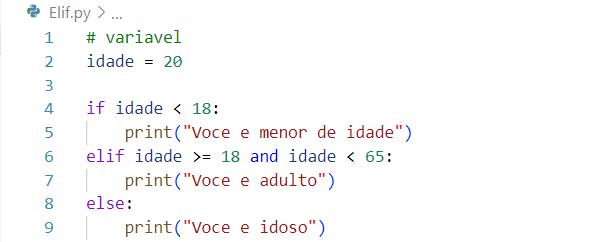
\includegraphics[width=12cm]{elif} 
		\newline
		Fonte: Criado por Mariana Cossetti Dalfior
	\end{center}
\end{figure}

\begin{figure}[H]
	\begin{center}
		\caption{Resultado do c\'{o}digo fonte do exemplo do uso do \textsl{elif}} \label{resulelif}
		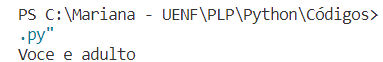
\includegraphics[width=9cm]{resulelif} 
		\newline
		Fonte: Criado por Mariana Cossetti Dalfior
	\end{center}
\end{figure}

%%%.........................................................................................%%%
            \subsection{La\c{c}o \textsl{For}}
%%%.........................................................................................%%%
O la\c{c}o "\textsl" \'{e} usado para iterar sobre uma sequ\^{e}ncia, sendo uma estrutura de controle de fluxo que repete um bloco de c\'{o}digo um determinado n\'{u}mero de vezes, at\'{e} atingir a condi\c{c}\~{a}o de parada. Al\'{e}m de que \'{e} poss\'{\i}vel combinar o \textsl{for} com outros comandos, como \textsl{if}, \textsl{else}, \textsl{break} e \textsl{continue}, para criar l\'{o}gicas mais complexas dentro do la\c{c}o. A sintaxe b\'{a}sica do la\c{c}o \textsl{for} em Python \'{e} a seguinte:

\begin{lstlisting}
>>> for <variavel> in <sequencia>:
>>> # bloco de codigo
\end{lstlisting}	

Durante cada itera\c{c}\~{a}o do la\c{c}o \textsl{for}, a vari\'{a}vel de itera\c{c}\~{a}o vai sendo incrementada, e o bloco de c\'{o}digo \'{e} executado com esse valor. O la\c{c}o continua at\'{e} que todos os itens da sequ\^{e}ncia tenham sido processados. A seguir \'{e} poss\'{\i}vel observar o c\'{o}digo fonte \ref{fontefor} e o resultado \ref{resulfor} do exemplo de um \textsl{for} em Python:

\begin{lstlisting}
>>> lista = [1, 2, 3, 4, 5]
>>> for v in lista:
>>> 	print(v)
1
2 
3
4
5
\end{lstlisting}	

\begin{figure}[H]
	\begin{center}
		\caption{C\'{o}digo fonte do exemplo do uso do \textsl{for}} \label{fontefor}
		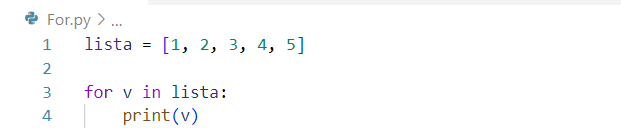
\includegraphics[width=12cm]{for} 
		\newline
		Fonte: Criado por Mariana Cossetti Dalfior
	\end{center}
\end{figure}

\begin{figure}[H]
	\begin{center}
		\caption{Resultado do c\'{o}digo fonte do exemplo do uso do \textsl{for}} \label{resulfor}
		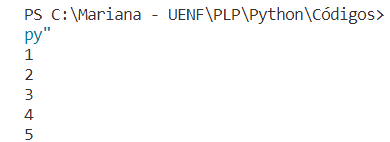
\includegraphics[width=9cm]{resulfor} 
		\newline
		Fonte: Criado por Mariana Cossetti Dalfior
	\end{center}
\end{figure}

%%%.........................................................................................%%%
            \subsection{La\c{c}o \textsl{While}}
%%%.........................................................................................%%%
O la\c{c}o de repeti\c{c}\~{a}o "\textsl{while}" \'{e} utilizado para repetir um bloco de c\'{o}digo at\'{e} uma condi\c{c}\~{a}o for falsa. A sua sintaxe geral em Python \'{e} a seguinte:

\begin{lstlisting}
>>> while condicao:
>>> # bloco de codigo a ser executado enquanto a condicao for 
>>> # verdadeira
\end{lstlisting}	

O bloco de c\'{o}digo dentro do la\c{c}o \textsl{while} vai ser executado diversas vezes at\'{e} que a condi\c{c}\~{a}o seja falsa. \'{E} necess\'{a}rio ter bastante cuidado para evitar a cria\c{c}\~{a}o de um loop infinito, pois a condi\c{c}\~{a}o nunca se torna falsa e ent\~{a}o o programa nunca parar\'{a} de ser executado. A seguir \'{e} poss\'{\i}vel observar o c\'{o}digo fonte \ref{fontewhile} e o resultado \ref{resulwhile} do exemplo de um laço \textsl{while} em Python:

\begin{lstlisting}
>>> # variaveis
>>> soma = 0
>>> v = 1
>>> 
>>> while v <= 10:
>>> 	soma += v
>>> 	v += 1
>>> print(soma)
55
\end{lstlisting}	

\begin{figure}[H]
	\begin{center}
		\caption{C\'{o}digo fonte do exemplo do uso do \textsl{while}} \label{fontewhile}
		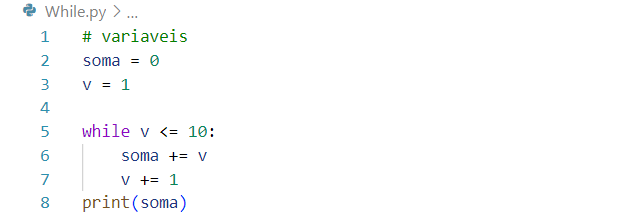
\includegraphics[width=12cm]{while} 
		\newline
		Fonte: Criado por Mariana Cossetti Dalfior
	\end{center}
\end{figure}

\begin{figure}[H]
	\begin{center}
		\caption{Resultado do c\'{o}digo fonte do exemplo do uso do \textsl{while}} \label{resulwhile}
		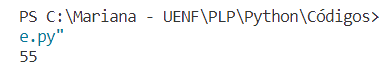
\includegraphics[width=9cm]{resulwhile} 
		\newline
		Fonte: Criado por Mariana Cossetti Dalfior
	\end{center}
\end{figure}